\documentclass[journal,12pt,twocolumn]{IEEEtran}

\usepackage{setspace}
\usepackage{gensymb}


\singlespacing

\usepackage[cmex10]{amsmath}
%\usepackage{amsthm}
%\interdisplaylinepenalty=2500
%\savesymbol{iint}
%\usepackage{txfonts}
%\restoresymbol{TXF}{iint}
%\usepackage{wasysym}
\usepackage{amsthm}

\usepackage{mathrsfs}
\usepackage{txfonts}
\usepackage{stfloats}
\usepackage{bm}
\usepackage{cite}
\usepackage{cases}
\usepackage{subfig}

\usepackage{longtable}
\usepackage{multirow}

\usepackage{enumitem}
\usepackage{mathtools}
\usepackage{steinmetz}
\usepackage{tikz}
\usepackage{circuitikz}
\usepackage{verbatim}
\usepackage{tfrupee}
\usepackage[breaklinks=true]{hyperref}

\usepackage{tkz-euclide} %loads TikZ and tkz-base

\usetikzlibrary{calc,math}
\usepackage{listings}
    \usepackage{color}                                          
    \usepackage{array}                                          
    \usepackage{longtable}                                      
    \usepackage{calc}                                           
    \usepackage{multirow}                                       
    \usepackage{hhline}                                         
    \usepackage{ifthen}
    \usepackage{lscape}     
\usepackage{multicol}
\usepackage{chngcntr}

\DeclareMathOperator*{\Res}{Res}

\renewcommand\thesection{\arabic{section}}
\renewcommand\thesubsection{\thesection.\arabic{subsection}}
\renewcommand\thesubsubsection{\thesubsection.\arabic{subsubsection}}

\renewcommand\thesectiondis{\arabic{section}}
\renewcommand\thesubsectiondis{\thesectiondis.\arabic{subsection}}
\renewcommand\thesubsubsectiondis{\thesubsectiondis.\arabic{subsubsection}}

\hyphenation{op-tical net-works semi-conduc-tor}
\def\inputGnumericTable{}                                 %%

\lstset{
%language=C,
frame=single, 
breaklines=true,
columns=fullflexible
}

\begin{document}

\newtheorem{theorem}{Theorem}[section]
\newtheorem{problem}{Problem}
\newtheorem{proposition}{Proposition}[section]
\newtheorem{lemma}{Lemma}[section]
\newtheorem{corollary}[theorem]{Corollary}
\newtheorem{example}{Example}[section]
\newtheorem{definition}[problem]{Definition}

\newcommand{\BEQA}{\begin{eqnarray}}
\newcommand{\EEQA}{\end{eqnarray}}
\newcommand{\define}{\stackrel{\triangle}{=}}

\bibliographystyle{IEEEtran}

\providecommand{\mbf}{\mathbf}
\providecommand{\pr}[1]{\ensuremath{\Pr\left(#1\right)}}
\providecommand{\qfunc}[1]{\ensuremath{Q\left(#1\right)}}
\providecommand{\sbrak}[1]{\ensuremath{{}\left[#1\right]}}
\providecommand{\lsbrak}[1]{\ensuremath{{}\left[#1\right.}}
\providecommand{\rsbrak}[1]{\ensuremath{{}\left.#1\right]}}
\providecommand{\brak}[1]{\ensuremath{\left(#1\right)}}
\providecommand{\lbrak}[1]{\ensuremath{\left(#1\right.}}
\providecommand{\rbrak}[1]{\ensuremath{\left.#1\right)}}
\providecommand{\cbrak}[1]{\ensuremath{\left\{#1\right\}}}
\providecommand{\lcbrak}[1]{\ensuremath{\left\{#1\right.}}
\providecommand{\rcbrak}[1]{\ensuremath{\left.#1\right\}}}
\theoremstyle{remark}
\newtheorem{rem}{Remark}
\newcommand{\sgn}{\mathop{\mathrm{sgn}}}
\providecommand{\abs}[1]{\left\vert#1\right\vert}
\providecommand{\res}[1]{\Res\displaylimits_{#1}} 
\providecommand{\norm}[1]{\left\lVert#1\right\rVert}
%\providecommand{\norm}[1]{\lVert#1\rVert}
\providecommand{\mtx}[1]{\mathbf{#1}}
\providecommand{\mean}[1]{E\left[ #1 \right]}
\providecommand{\fourier}{\overset{\mathcal{F}}{ \rightleftharpoons}}
%\providecommand{\hilbert}{\overset{\mathcal{H}}{ \rightleftharpoons}}
\providecommand{\system}{\overset{\mathcal{H}}{ \longleftrightarrow}}
	%\newcommand{\solution}[2]{\textbf{Solution:}{#1}}
\newcommand{\solution}{\noindent \textbf{Solution: }}
\newcommand{\cosec}{\,\text{cosec}\,}
\providecommand{\dec}[2]{\ensuremath{\overset{#1}{\underset{#2}{\gtrless}}}}
\newcommand{\myvec}[1]{\ensuremath{\begin{pmatrix}#1\end{pmatrix}}}
\newcommand{\mydet}[1]{\ensuremath{\begin{vmatrix}#1\end{vmatrix}}}

\numberwithin{equation}{subsection}

\makeatletter
\@addtoreset{figure}{problem}
\makeatother

\let\StandardTheFigure\thefigure
\let\vec\mathbf

\renewcommand{\thefigure}{\theproblem}

\def\putbox#1#2#3{\makebox[0in][l]{\makebox[#1][l]{}\raisebox{\baselineskip}[0in][0in]{\raisebox{#2}[0in][0in]{#3}}}}
     \def\rightbox#1{\makebox[0in][r]{#1}}
     \def\centbox#1{\makebox[0in]{#1}}
     \def\topbox#1{\raisebox{-\baselineskip}[0in][0in]{#1}}
     \def\midbox#1{\raisebox{-0.5\baselineskip}[0in][0in]{#1}}
\vspace{3cm}

\title{Challenging Problem 1}
\author{Surbhi Agarwal}

\maketitle

\newpage

%\tableofcontents

\bigskip

\renewcommand{\thefigure}{\theenumi}
\renewcommand{\thetable}{\theenumi}

\begin{abstract}
This document shows the method to find the closest points on two skew lines in 3-Dimension.
\end{abstract}

Download all python codes from 
%
\begin{lstlisting}
https://github.com/surbhi0912/EE5609/tree/master/challenging_problem/challenging1/codes
\end{lstlisting}
%
and latex-tikz codes from 
%
\begin{lstlisting}
https://github.com/surbhi0912/EE5609/tree/master/challenging_problem/challenging1
\end{lstlisting}
%
\section{Problem}
In 3-Dimensional Space, find the points on the two skew lines
\begin{align}\label{eqn1}
    L_1 : \vec{x} = \myvec{1 \\ 1 \\ 0} + \lambda_1\myvec{2 \\ -1 \\ 1}
\end{align}
\begin{align}\label{eqn2}
    L_2 : \vec{x} = \myvec{2 \\ 1 \\ -1} + \lambda_2\myvec{3 \\ -5 \\2}
\end{align}
such that the points are closest to each other
\section{Solution}
In the given problem,
\begin{align}\label{e3}
    \vec{A}_1 = \myvec{1 \\ 1 \\ 0}, \vec{m}_1 = \myvec{2 \\ -1 \\ 1}, \vec{A}_2 = \myvec{2 \\ 1 \\ -1}, \vec{m}_2 = \myvec{3 \\ -5 \\ 2}
\end{align}
where $L_1$ is passing through the point $A_1(1,1,0)$ and direction vector $\vec{m}_1$,\\
And $L_2$ is passing through the point $A_2(2,1,-1)$ and direction vector $\vec{m}_2$

Let us take a point $\vec{E}$ on Line $L_1$ and $\vec{F}$ on Line $L_2$ such that they are closest to each other.

Then $\vec{E}$ and $\vec{F}$ can be expressed using Equation $\ref{eqn1}$ and $\ref{eqn2}$ respectively as follows :
\begin{align}
    \vec{E} = \myvec{1 \\ 1 \\ 0} + \lambda_1\myvec{2 \\ -1 \\ 1}
\end{align}
\begin{align}
    \vec{F} = \myvec{2 \\ 1 \\ -1} + \lambda_2\myvec{3 \\ 5 \\ -2}
\end{align}
Now, the position vector from $\vec{E}$ to $\vec{F}$, ie $\vec{F}-\vec{E}$ is given as,
\begin{align}
    \vec{F}-\vec{E} & = (\vec{A}_2 + \lambda_2\vec{m}_2) - (\vec{A}_1 + \lambda_1\vec{m}_1)\\& = (\vec{A}_2 - \vec{A}_1) + (\lambda_2\vec{m}_2 - \lambda_1\vec{m}_1)
\end{align}
\begin{align}
    \implies\vec{F}-\vec{E} & = \myvec{2 \\ 1 \\ -1}-\myvec{1 \\ 1 \\ 0} + \lambda_2\myvec{3 \\ -5 \\ 2} -\lambda_1\myvec{2\\-1\\1}\\&=\myvec{1\\ 0 \\ -1}+ \lambda_2\myvec{3 \\ -5 \\ 2} +\lambda_1\myvec{-2\\1\\-1}\\& = \label{e4} \myvec{1\\ 0 \\ -1}+\myvec{3&-2\\-5&1\\2&-1}\myvec{\lambda_2 \\ \lambda_1} 
\end{align}
Since the points $\vec{E}$ and $\vec{F}$ are closest to each other, position vector $\vec{F}-\vec{E}$ is perpendicular to the skew lines $L_1$ and $L_2$, thus we can say that $\vec{F}-\vec{E}$ is perpendicular to the direction vectors of these lines, ie $\vec{m}_1$ and $\vec{m}_2$ respectively. Therefore,
\begin{align}\label{e5}
    \vec{m}_1^T(\vec{F}-\vec{E}) = 0
\end{align}
\begin{align}\label{e6}
    \vec{m}_2^T(\vec{F}-\vec{E}) = 0
\end{align}
Using the values of $\vec{F}-\vec{E}$, $\vec{m}_1$, $\vec{m}_2$ from Equations \ref{e4} and \ref{e3} in Equations \ref{e5} and \ref{e6},
\begin{align}\label{e7}
    \myvec{2 \\ -1 \\ 1}^T\left(\myvec{1\\ 0 \\ -1}+\myvec{3&-2\\-5&1\\2&-1}\myvec{\lambda_2 \\ \lambda_1}\right) = 0
\end{align}
\begin{align}\label{e8}
    \myvec{3 \\ -5 \\ 2}^T\left(\myvec{1\\ 0 \\ -1}+\myvec{3&-2\\-5&1\\2&-1}\myvec{\lambda_2 \\ \lambda_1}\right) = 0
\end{align}
Expanding Equations \eqref{e7}, \eqref{e8}
\begin{align}
    \myvec{2&-1& 1}\myvec{1\\0\\-1} +\lambda_2\myvec{2&-1&1}\myvec{3\\-5\\2}+ \lambda_1\myvec{2&-1&1}\myvec{-2\\1\\-1}= 0 \\
    \myvec{3&-5&2}\myvec{1\\0\\-1} +\lambda_2\myvec{3&-5&2}\myvec{3\\-5\\2}+\lambda_1\myvec{3&-5&2}\myvec{-2\\1\\-1}= 0
\end{align}
This gives us,
\begin{align}\label{e9}
    6\lambda_1 -13\lambda_2 = 1
\end{align}
\begin{align}\label{e10}
   13\lambda_1 -38\lambda_2 = 1
\end{align}
Solving Equation \ref{e9} and \ref{e10}, $\lambda_1 = \dfrac{25}{59}$ and $\lambda_2 = \dfrac{7}{59}$\\
\begin{align}
    \vec{E} & = \myvec{\frac{109}{59} \\ \frac{34}{59}
    \\ \frac{25}{59}}
    \\&=\myvec{1.85 \\ 0.58 \\ 0.42}
\end{align}
\begin{align}
    \vec{F} & = \myvec{\frac{139}{59} \\ \frac{24}{59}
    \\ \frac{-45}{59}}
    \\&=\myvec{2.36 \\ 0.41 \\ -0.76}
\end{align}
\\
The figure obtained is shown in Fig \ref{myfig}
\renewcommand{\thefigure}{1}
\begin{figure}[h!]
    \centering
    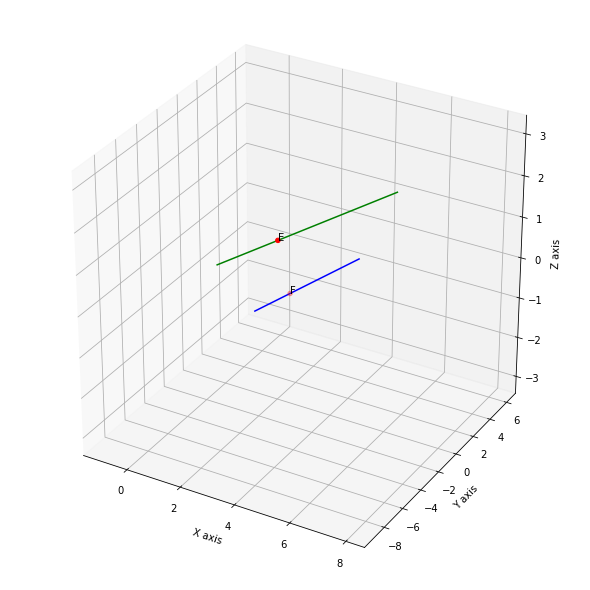
\includegraphics[width=\columnwidth]{closest.png}
    \caption{Closest points between skew lines $L_1$ and $L_2$}
    \label{myfig}
\end{figure}
\end{document}